%% LyX 2.0.3 created this file.  For more info, see http://www.lyx.org/.
%% Do not edit unless you really know what you are doing.
\documentclass[usenatbib]{mn2e}
\usepackage[latin9]{inputenc}
\usepackage[a4paper]{geometry}
\geometry{verbose}
\setcounter{tocdepth}{3}
\usepackage{color}
\usepackage{float}
\usepackage{graphicx}

\makeatletter

%%%%%%%%%%%%%%%%%%%%%%%%%%%%%% LyX specific LaTeX commands.
%% Because html converters don't know tabularnewline
\providecommand{\tabularnewline}{\\}
%% A simple dot to overcome graphicx limitations
\newcommand{\lyxdot}{.}


%%%%%%%%%%%%%%%%%%%%%%%%%%%%%% User specified LaTeX commands.






%%%%%%%%%%%%%%%%%%%%%%%%%%%%%% LyX specific LaTeX commands.
%% A simple dot to overcome graphicx limitations
%Make my life significantly easier

\global\long\def\bd{{\bm{\delta}}}

\makeatother

\begin{document}
We are interested in recovering the halos and their masses, positions
and velocities with the smallest time step necessary to preserve sufficient
properties as mock catalogs.


\section{Matching Halos}

First, we compare a halo by halo in different simulations. Since all
the simulations use exactly the same initial conditions, if those
approximated N-body simulations can recover the halos reasonably well
(compared to a full N-body simulation), then we should find the same
halo at the same position with the same mass in different samples.
The question here are how mass resolutions and time steps affect on
halo properties (i.e., mass, position and velocity) and how many halos
don't correspond to halos in different samples.

To spatially match the halos defined in different mass resolution
and time step parameters, we first find a pair of halos from two different
simulations, whose distance is the closest. Then, we set two conditions
on those pairs to declare that those paired halos are the same halos:

1) distance is smaller than $0.5h^{-1}{\rm Mpc}$,

2) mass ratio is smaller than $10^{0.5}{\rm M_{\odot}}$.

Under the above conditions, \textcolor{black}{more than}\textcolor{red}{{}
}90\% of halos in 450/5 found paired halos in 300/2 at redshift $z=0.15$
with a fixed mass resolution, $256^{3}$ particles (shown in \textcolor{black}{Table}\textcolor{red}{{}
}\ref{tab:unmatchedHalo}). We also checked how those conditions affect
to fraction of matched halos by changing the numerical values for
distance and mass ratio criteria. As shown in Table \ref{tab:unmatchedHalo},
changing a criterion on mass ratio did not change the fraction compared
to the distance criterion. This indicates that deviation of halo masses
on pairs is relatively small.

\begin{table*}[p]
\begin{tabular}{|c|c|c|c|}
\hline 
mass$[{\rm M_{\odot}]}$\textbackslash{}distance $[h^{-1}{\rm Mpc}]$ & 0.5 & 0.75 & 1.0\tabularnewline
\hline 
\hline 
$10^{0.5}$ & 0.0915 & 0.0842 & 0.0842\tabularnewline
\hline 
$10^{0.75}$ & 0.0909 & 0.0825 & 0.0817\tabularnewline
\hline 
$10^{1.0}$ & 0.0909 & 0.0823 & 0.0763\tabularnewline
\hline 
\end{tabular}

\caption{\label{tab:unmatchedHalo}Fractions of unmatched halos (over matched
halos) for the sample of 450/5 when we compare a halo by halo for
300/2 at redshift $z=0.15$. Here, both simulations have the same
mass resolution (i.e., $256^{3}$ particles in the box of $(256h^{-1}{\rm Mpc})^{3}$).
This table shows how the fraction is changed according to changing
the matching conditions for distance and mass ratio.}


\end{table*}



\subsection{Mass Resolution}

In this section, we examine how mass resolutions affect to halo properties.
We use a $(256h^{-1}{\rm Mpc)^{3}}$-cubical box and three different
mass resolutions: $512^{3}$, $256^{3}$, and $128^{3}$ particles
with a fixed time steps (450/5). We take a simulation of $512^{3}$
particles as a reference. Table \ref{tab:unmatched_512} indicates
fractions of unmatched halos in the sample of $512^{3}$-particle
mass resolution by matching with the samples of $256^{3}$ and $128^{3}$
particles at redshift $z=0.15$. Since having a different mass resolution
means that halo samples have different lower mass limits, we only
impose matching conditions on halos greater than $10^{12.5}{\rm M_{\odot}}$
for the $256^{3}$-particles sample and greater than $10^{13.5}{\rm M_{\odot}}$for
the $128^{3}$-particles sample. \textcolor{red}{XXXX}

\begin{table*}[p]
\begin{tabular}{|c|c|c|c|}
\hline 
mass-resolution\textbackslash{}z & 0.15 & 0.5 & 0.8\tabularnewline
\hline 
\hline 
$256^{3}$ & 0.872 & 0.879 & 0.889\tabularnewline
\hline 
$128^{3}$ & 0.997 & 0.998 & 0.998\tabularnewline
\hline 
\end{tabular}

\caption{\label{tab:unmatched_512}(WRONG!!!!!!!!!)Fractions of unmatched halos
(over matched halos) for the sample of $512^{3}$ particles when we
compare a halo by halo for $256^{3}$ and $128^{3}$ particles with
a fixed time step (450/5). Most of halos are unmatched due to large
differences on numbers of halo in different mass resolution samples.}
\end{table*}


\begin{figure*}
\includegraphics[width=1\columnwidth]{/Users/ts485/Dropbox/Tomomi/HACC/Conv/Matching_halos/plots_450_5/unmatchedHalo_256_450_5_z0\lyxdot 15}\includegraphics[width=1\columnwidth]{/Users/ts485/Dropbox/Tomomi/HACC/Conv/Matching_halos/plots_450_5/unmatchedHalo_128_450_5_z0\lyxdot 15}

\caption{\label{fig:unmatchedHalo512}Unmatched halo number density for the
simulation of $512^{3}$ particles (blue in both panels) by comparing
with $256^{3}$ particles-simulation (left, green) and $128^{3}$-particles
simulation (right, green) at redshift $z=0.15$. }
\end{figure*}


Figure \ref{fig:unmatchedHalo512} shows number densities of unmatched
halos as a function of halo mass at redshift $z=0.15$. In matching,
an algorithm takes a finer resolution sample as a reference and finds
a matched halo from the other sample. Surprisingly, the number densities
for bothe samples are almost the same. We use a mass treshold of $10^{12.5}{\rm M_{\odot}}$
for the comparison between $512^{3}$ and $256^{3}$ particles samples
and $10^{13.5}{\rm M_{\odot}}$ for $512^{3}$ and $128^{3}$ particles
samples.

\begin{figure*}
\includegraphics[width=1\columnwidth]{/Users/ts485/Dropbox/Tomomi/HACC/Conv/Matching_halos/plots_450_5/distance1_normed_450_5_z0\lyxdot 15} 

\caption{\label{fig:HaloPosition512}Histograms of distance difference for
matched halos with respect to halos from $512^{3}$ particles with
450 large steps and 5 inner steps. Different colors correspond to
different mass resolutions: $256^{3}$ particles and $128^{3}$ particles
with a fixed time step (450/5) at redshift $z=0.15$. }


\end{figure*}


Figure \ref{fig:HaloPosition512} depicts the halo position differences
of individual halos. The simulation with $128^{3}$ particles has
more scatter and its distribution is not Gaussian ($\rightarrow$
\textcolor{red}{What does this possibly imply? How does this affect
to power spectra?}). For the simulation with $256^{3}$ particles,
the result improves siginificantly and the positions are matched within
a few hundreds kpc. For halo masses, the results are shown in Figure
\ref{fig:HaloMass512} and both simulations with $256^{3}$ and $128^{3}$
particles well agree with the simulation with $512^{3}$ particles.

\begin{figure*}
\includegraphics[width=1\columnwidth]{/Users/ts485/Dropbox/Tomomi/HACC/Conv/Matching_halos/plots_450_5/histogram3_normed_450_5_z0\lyxdot 15}

\caption{\label{fig:HaloMass512}Histograms of log-based mass difference for
different mass resolutions with respect to $512^{3}$ particles at
redshift $z=0.15$. Histograms are normalized and all simulations
have the same time step, 450/5. Colors correspond to $256^{3}$ particles
(blue) and $128^{3}$ particles (green).}


\end{figure*}


\begin{figure*}
\includegraphics[width=1\columnwidth]{/Users/ts485/Dropbox/Tomomi/HACC/Conv/Matching_halos/plots_450_5/velMag1_normed_450_5_z0\lyxdot 15}

\caption{\label{fig:HaloVelocity512}Histograms of velocity magnitude difference
for matched halos with respect to halos from $512^{3}$ particles
at redshift $z=0.15$. Different colors correspond to different mass
resolutions: $256^{3}$ particles (blue) and $128^{3}$ particles
(green). All the simulations use the same step size, 450/5. Note that
angle difference of velocity vectors for 95\% of matched halos in
the $256^{3}$-particle sample are within 0.3 radians and 90\% in
the $128^{3}$-particle sample are within 0.6 radians.}


\end{figure*}


Figure \ref{fig:HaloVelocity512} indicates that difference on velocity
magnitude for $256^{3}$-particles sample is relatively small.


\subsection{Time steps}

In this section, we examine how global steps and sub-cycles affect
to halo properties. The goal here is to know the smallest global steps
and sub-cycles required to preserve necessary properties as mocks. 

Here, all the samples have the same mass resolution, $256^{3}$ particles
in the box of $(256h^{-1}{\rm Mpc})^{3}$. We use 450/5 (450 global
steps and 5 sub-cycles) as a reference to other samples: 300/3, 300/2,
150/3, and 150/2.

\begin{figure*}
\includegraphics[width=1\columnwidth]{/Users/ts485/Dropbox/Tomomi/HACC/Conv/Matching_halos/Distance/distance_z0\lyxdot 15}

\caption{\label{fig:HaloPosition}Histograms of distance difference for matched
halos with respect to halos from $256^{3}$ particles with 450 large
steps and 5 inner steps. Different colors correspond to different
simulation step sizes: 300 large steps with 3 inner steps (blue) and
2 inner steps (green), and 150 large steps with 3 inner steps (red)
and 2 inner steps (cyan). All the simulations use $256^{3}$ particles
at redshift $z=0.15$.}
\end{figure*}
 
\begin{table*}[H]
\begin{tabular}{|c|c|c|}
\hline 
z=0.15 & mean {[}$h^{-1}{\rm Mpc}${]} & std{[}$(h^{-1}{\rm Mpc)^{2}}${]}\tabularnewline
\hline 
\hline 
300/3 & 0.078 & 0.056\tabularnewline
\hline 
300/2 & 0.092 & 0.068\tabularnewline
\hline 
150/3 & 0.233 & 0.106\tabularnewline
\hline 
150/2 & 0.237 & 0.107\tabularnewline
\hline 
\end{tabular}%
\begin{tabular}{|c|c|c|}
\hline 
z=0.5 & mean {[}$h^{-1}{\rm Mpc}${]} & std{[}$(h^{-1}{\rm Mpc)^{2}}${]}\tabularnewline
\hline 
\hline 
300/3 & 0.078 & 0.053\tabularnewline
\hline 
300/2 & 0.089 & 0.062\tabularnewline
\hline 
150/3 & 0.196 & 0.095\tabularnewline
\hline 
150/2 & 0.202 & 0.097\tabularnewline
\hline 
\end{tabular}%
\begin{tabular}{|c|c|c|}
\hline 
z=0.8 & mean {[}$h^{-1}{\rm Mpc}${]} & std{[}$(h^{-1}{\rm Mpc)^{2}}${]}\tabularnewline
\hline 
\hline 
300/3 & 0.068 & 0.050\tabularnewline
\hline 
300/2 & 0.080 & 0.059\tabularnewline
\hline 
150/3 & 0.199 & 0.096\tabularnewline
\hline 
150/2 & 0.204 & 0.097\tabularnewline
\hline 
\end{tabular}

\caption{\label{tab:HaloPosition}Means and standard deviations for positional
differences in Figure \ref{fig:HaloPosition}.}


\end{table*}


Figure \ref{fig:HaloPosition} shows the halo position differences
of paired halos as distances. This histogram indicates that global
step has bigger effects on overall halo positions and different sub-cycles
have negligible effects. Most of halos for 300 global steps have their
center positions within 100 kpc with respect to halo center positions
for 450/5, while the simulations for 150 global steps have more scatter
in the figure. Means and standard deviations for the histograms are
shown in Table \ref{tab:HaloPosition}.

\begin{figure*}
\includegraphics[width=1\columnwidth]{/Users/ts485/Dropbox/Tomomi/HACC/Conv/Matching_halos/Histogram/histogram3_diff_z0\lyxdot 15}

\caption{\label{fig:HaloMass}Histograms of log-based mass difference of different
simulation step sizes with respect to the one with 450 large steps
and 5 inner steps. Histograms are not normalized and all halos are
from the simulations with $256^{3}$ particles. For each of simulations:
300 large steps with 3 inner steps (blue) and 2 inner steps (green),
and 150 large steps with 3 inner steps (red).}


\end{figure*}


\begin{table*}
\begin{tabular}{|c|c|c|}
\hline 
z=0.15 & mean & std\tabularnewline
\hline 
\hline 
300/3 & -0.005 & 0.067\tabularnewline
\hline 
300/2 & -0.011 & 0.075\tabularnewline
\hline 
150/3 & -0.035 & 0.074\tabularnewline
\hline 
150/2 & -0.059 & 0.087\tabularnewline
\hline 
\end{tabular}%
\begin{tabular}{|c|c|c|}
\hline 
z=0.5 & mean & std\tabularnewline
\hline 
\hline 
300/3 & -0.007 & 0.069\tabularnewline
\hline 
300/2 & -0.019 & 0.075\tabularnewline
\hline 
150/3 & -0.047 & 0.082\tabularnewline
\hline 
150/2 & -0.078 & 0.091\tabularnewline
\hline 
\end{tabular}%
\begin{tabular}{|c|c|c|}
\hline 
z=0.8 & mean & std\tabularnewline
\hline 
\hline 
300/3 & -0.009 & 0.069\tabularnewline
\hline 
300/2 & -0.026 & 0.077\tabularnewline
\hline 
150/3 & -0.065 & 0.084\tabularnewline
\hline 
150/2 & -0.100 & 0.094\tabularnewline
\hline 
\end{tabular}

\caption{\label{tab:HaloMass}Means and standard deviations for halo mass differences
in log-based halo mass (with base 10) in Figure \ref{fig:HaloMass}. }


\end{table*}


Figure \ref{fig:HaloMass} shows halo mass differences for paired
halos with respect to halos from 450/5. Global steps affect on overall
distribution properties (i.e., mean and standard deviation shown in
Table \ref{tab:HaloMass}), while sub-cycles affect on their amplitudes.
This is because sub-cycles changes small-scale dynamics and it can
cause a difference on number of halos declared through FOF, whose
linking length is fixed to $b=0.2$. In general, smaller step sizes
make distribution of DM particles as halos more diffused (since smaller
stepsizes means that dynamics is more linear(?)) and there is a possibility
that some of gathered DM particles are not considered as halos. In
\textcolor{red}{Manera et al.} which approximates N-body simulations
by using the second-order Lagrangian Perturbation Theory, they solved
this problem by changing the linking length for FOF. ->\textcolor{red}{{}
Can we tune (or do we need to tune) linking lengths based on step
sizes?}

\begin{figure*}[p]
\includegraphics[width=1\columnwidth]{/Users/ts485/Dropbox/Tomomi/HACC/Conv/Plots4lyx/velMag_z0\lyxdot 15}

\caption{\label{fig:HaloVelocity}Histograms of velocity magnitude difference
for matched halos with respect to halos from $256^{3}$ particles
with 450 large steps and 5 inner steps. Different colors correspond
to different simulation stepsizes: 300 large steps with 3 inner steps
(blue) and 2 inner steps (green), and 150 large steps with 3 inner
steps (red) and 2 inner steps (cyan). All the simulations use $256^{3}$
particles at redshift $z=0.15$. Note that angle difference of velocity
vectors for 98\% of matched halos are within 0.3 radians.}
\end{figure*}
 
\begin{table}
\begin{tabular}{|c|c|c|}
\hline 
z=0.15 & mean {[}${\rm km/{\rm s}}${]} & std {[}$({\rm km/{\rm s})^{2}}${]}\tabularnewline
\hline 
\hline 
300/3 & -3.54 & 23.27\tabularnewline
\hline 
300/2 & -3.90 & 25.65\tabularnewline
\hline 
150/3 & -17.77 & 28.83\tabularnewline
\hline 
150/2 & -17.94 & 29.30\tabularnewline
\hline 
\end{tabular}%
\begin{tabular}{|c|c|c|}
\hline 
z=0.5 & mean {[}${\rm km/{\rm s}}${]} & std {[}$({\rm km/{\rm s})^{2}}${]}\tabularnewline
\hline 
\hline 
300/3 & -4.36 & 33.23\tabularnewline
\hline 
300/2 & -4.07 & 34.54\tabularnewline
\hline 
150/3 & -25.30 & 40.72\tabularnewline
\hline 
150/2 & -26.34 & 42.26\tabularnewline
\hline 
\end{tabular}%
\begin{tabular}{|c|c|c|}
\hline 
z=0.8 & mean {[}${\rm km/{\rm s}}${]} & std {[}$({\rm km/{\rm s})^{2}}${]}\tabularnewline
\hline 
\hline 
300/3 & -6.37 & 39.96\tabularnewline
\hline 
300/2 & -6.66 & 42.77\tabularnewline
\hline 
150/3 & -26.11 & 51.25\tabularnewline
\hline 
150/2 & -27.83 & 54.28\tabularnewline
\hline 
\end{tabular}

\caption{\label{tab:HaloVelocity}Means and standard deviations for halo velocity
differences in Figure \ref{fig:HaloVelocity}.}


\end{table}


For halo velocities, the results are shown in Figure \ref{fig:HaloVelocity}.
The histogram is a function of velocity magnitude differences. For
150 global steps, the means slightly deviate from 0 and have negative
values. This means that magnitude of velocity for 150 global steps
is smaller than that for 450 global steps. One way to explain about
it is that because smaller time step halos are less dense, the potential
wells at center of halos may be less deeper than the ones for larger
step sizes. We also examined differences on velocity direction (orientation?).
More than 98\% of paired halos have angle differences (with respect
to halos for 450/5) within 0.3 radians. This implies that orientation
of velocities are well-preserved among the samples for different time
steps.

\begin{figure*}
\includegraphics[width=1\columnwidth]{/Users/ts485/Dropbox/Tomomi/HACC/Conv/Plots4lyx/New_unmatchedHalo_256_300_2_z0\lyxdot 15}\includegraphics[width=1\columnwidth]{/Users/ts485/Dropbox/Tomomi/HACC/Conv/Plots4lyx/New_unmatchedHaloRatio_256_z0\lyxdot 15}

\caption{\label{fig:unmatchedHalo}Upper: Unmatched halo number density for
the simulation of 300 large steps and 2 inner steps matching with
450 large steps and 5 inner steps. Both are from $256^{3}$ particle
simulations. Lower: Ratio of unmatched halo number densities (which
are the same as the ones in the left plot) with respect to the corresponding
total number densities. Both plots are at redshift $z=0.15$. I am
not sure why there are more unmatched halos above $10^{14}{\rm M_{\odot}}$
for 150/2. -> I may check the conditions of surrounding halos...}
\end{figure*}
 
\begin{table*}[p]
\begin{tabular}{|c|c|c|c|}
\hline 
time step/z & 0.15 & 0.5 & 0.8\tabularnewline
\hline 
\hline 
300/3 & 0.099 & 0.107 & 0.120\tabularnewline
\hline 
300/2 & 0.134 & 0.154 & 0.182\tabularnewline
\hline 
150/3 & 0.219 & 0.233 & 0.285\tabularnewline
\hline 
150/2 & 0.299 & 0.331 & 0.387\tabularnewline
\hline 
\end{tabular}

\caption{\label{tab:unmatched_256}Fractions of unmatched halos (over matched
halos) for the sample of 450/5 when we compare a halo by halo for
other time steps shown in the table with a fixed mass resolution ($256^{3}$
particles). }
\end{table*}


At last, we show number density of unmatched halos in Figure \ref{fig:unmatchedHalo}
and Table \ref{tab:unmatched_256}. \textcolor{red}{Table \ref{tab:unmatched_256}
shows fractions of unmatched halos for the sample of 450/5 compared
with other time steps. Note that even though we only show the fractions
for 450/5, the fractions for other time steps correspond to the ones
for 450/5, as shown in Figure \ref{fig:unmatchedHalo}, which indicates
that number densities for unmatched halos are almost the same.} There
are more unmatched halos for smaller halo masses shown in the upper
panel of Figure \ref{fig:unmatchedHalo}, which compares 450/5 and
300/2 samples. When we find a matched halo in two different samples,
an algorithm tries to find a matched halo in a smaller step size sample
(for the case of the upper panel of Figure \ref{fig:unmatchedHalo},
300/2) for a larger step size sample (i.e., 450/5), and yet the number
densities for unmatched halos for both samples are almost the same
(which I somehow feel a little bit strange...). Unmatched number densities
for different step sizes are shown in the lower panel of Figure \ref{fig:unmatchedHalo}.
As is clear, sub-cycles in the number of unmatched halos is negligible.
Again, changing the matching conditions don't affect on the fraction
of unmatched halos much and the fraction is always less than 10\%.

{*}{*}{*}snapshots for unmatched halos whose mass is greater than
$10^{14}{\rm M_{\odot}}$

There are two unmatched halos whose mass is greater than $10^{14}{\rm M_{\odot}}$
in 450/5. One of them was completely unmatched with any halos from
300/2 (shown in Figure \ref{unmatch1}), while the other was due to
the distance criteion on matching conditions (shown in Figure \ref{unmatch2}).

\begin{figure*}[t]
\includegraphics[width=1\columnwidth]{/Users/ts485/Dropbox/Tomomi/HACC/Conv/Matching_halos/Unmatched_revised/mass14_unmacthedHalo1_data}\includegraphics[width=1\columnwidth]{/Users/ts485/Dropbox/Tomomi/HACC/Conv/Matching_halos/Unmatched_revised/mass14_cont_unmatchedHalo1_sample}

\caption{\label{unmatch1}Two halos from 300/2 which are close to the unmatched
halo with halo mass $10^{14.003}{\rm M_{\odot}}$(from 450/5) are
separate more than $2h^{-1}{\rm Mpc}$ and are either larger ($10^{14.612}{\rm M_{\odot}})$
or smaller ($10^{13.3}{\rm M_{\odot}}$) than the mass criterion.}
\end{figure*}


\begin{figure*}[p]
\includegraphics[width=1\columnwidth]{/Users/ts485/Dropbox/Tomomi/HACC/Conv/Matching_halos/Unmatched_revised/mass14_unmacthedHalo2_data}\includegraphics[width=1\columnwidth]{/Users/ts485/Dropbox/Tomomi/HACC/Conv/Matching_halos/Unmatched_revised/mass14_cont_unmatchedHalo2_sample}

\caption{\label{unmatch2}This halo is considered as an unmatched halo, because
the closest halo from 300/2 has the distance of $0.55h^{-1}{\rm Mpc}$
(and log-mass difference of 0.1). The matching condition used here
was $0.5h^{-1}{\rm Mpc}$. }
\end{figure*}


Now, \textcolor{red}{we check the first halo more closely to investigate
why there is no declared halos}...


\section{Observable/Statistics}

Goal: To correctly describe the large-scale distribution of these
galaxies. $\Rightarrow$ Need to correctly locate DM halos in the
simulations and estimate their masses.


\subsection{Mass Function}

{*} Why do we care about mass functions?

{*} If we have samples with different mass functions, what does it
mean? and what kind of problems are caused by that?

{*} What does it physically (observationally?) mean to have the same
mass function?

{*} I am not sure how Manera et al. assigned masses to halos...apparently,
they were using analytic mass functions for this...:(


\subsubsection{Mass Resolution}

\begin{figure}
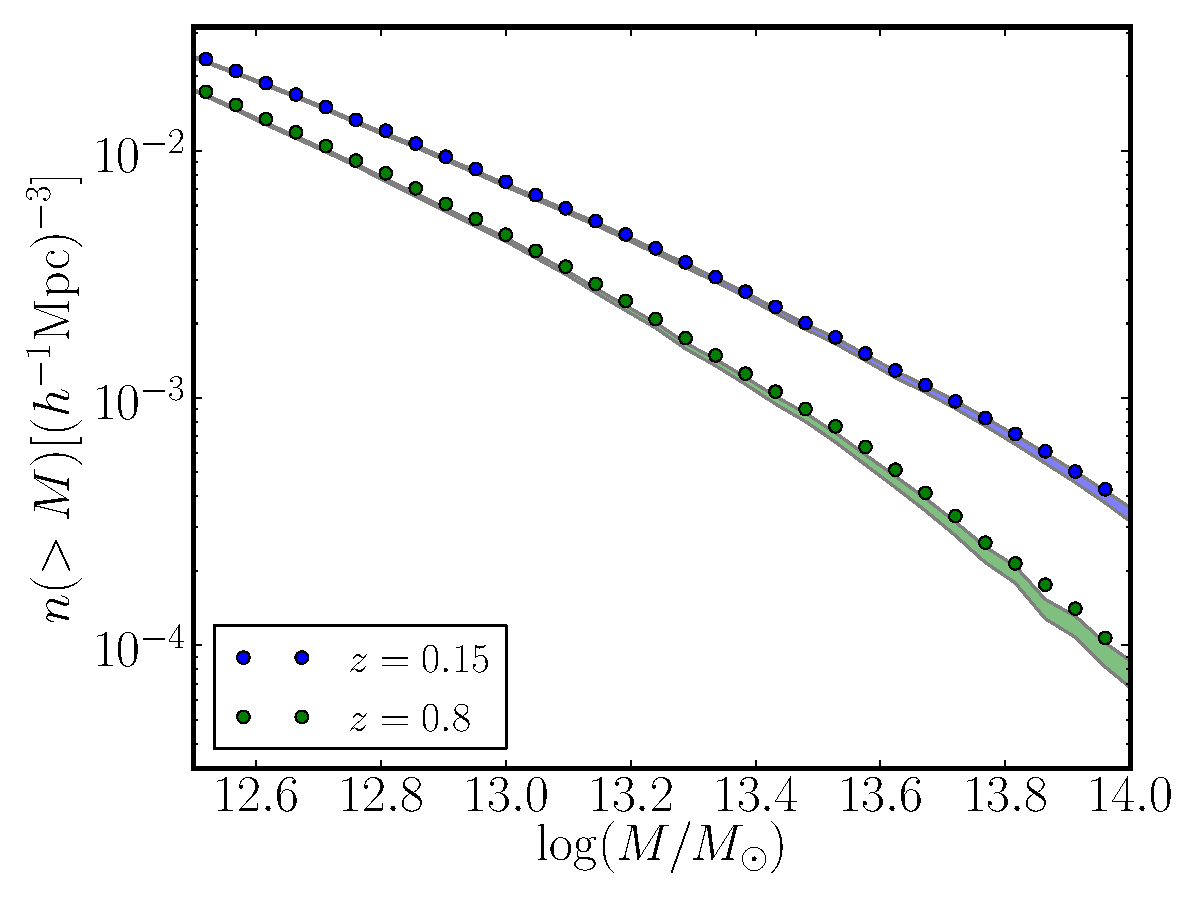
\includegraphics[width=1\columnwidth]{/Users/ts485/Dropbox/Tomomi/HACC/Conv/Plots4lyx/haloNum_massResolution}

\caption{Comparison of mass functions (should I call this number density?)
for different simulations at redshift $z=0.15$ and $z=0.8$. The
shaded regions indicate the upper limit and the lower limit of mass
functions for the simulation with $512^{3}$ particles and 450 steps
with 5 inner steps. The mean and standard deviations are calculated
from bootstrap method. We compare them with the simulations of $256^{3}$
particles with 450 large steps and 5 inner steps (described as $256^{3}$
with circles in the figure) and $128^{3}$ particles with 450 large
steps and 5 inner steps (described as $128^{3}$ with red stars in
the figure).}
\end{figure}



\subsubsection{Time Steps}

\begin{figure}
\includegraphics[width=1\columnwidth]{/Users/ts485/Dropbox/Tomomi/HACC/Conv/Plots4lyx/haloNum2}

\caption{Comparison of mass functions (should I call this number density?)
for different simulations at redshift $z=0.15$ and $z=0.8$. The
shaded regions indicate the upper limit and the lower limit of mass
functions for the simulation with $512^{3}$ particles and 450 steps
with 5 inner(?) steps. The mean and standard deviations are calculated
from bootstrap method. We compare them with the simulations of $256^{3}$
particles with 450 large steps and 5 inner steps (described as $256^{3}(450:5)$
with circles in the figure) and with 300 large steps and 2 inner steps
(described as $256^{3}(300:2)$ with red stars in the figure).}


\end{figure}


\begin{figure}
\includegraphics[width=1\columnwidth]{/Users/ts485/Dropbox/Tomomi/HACC/Conv/Plots4lyx/haloRatioNum256_z0\lyxdot 15}\caption{Ratios of mass functions of different time steps with $256^{3}$ particles,
compared to $512^{3}$ particles with 450 large steps and 5 inner
steps, at redshift $z=0.15$. Different colors are corresponding to
different time steps. The legend in the plot has the same format as
the one in Figure 1. This plot shows that the simulations with 450
and 300 large steps agree well with the simulation with $512^{3}$
particles.}
\end{figure}



\subsection{Halo power spectra}

From proporsal: ``A large enough number for the global time steps
is important to resolve the large scale structure correctly and recover,
e.g. the power spectrum correctly on large scales while the sub-cycles
mainly influence the inner structure of halos and the power spectrum
on the smallest scale.''

What we want to know here is quantitative effects of mass resolutions
and time steps on power spectra.


\subsubsection{Mass Resolution}

{*}only auto power spectra since I don't have DM particle samples
for $512^{3}$ particles resolution. Are there any meanings to calculate
cross-power with $256^{3}$ particles?

\begin{figure}
\includegraphics[width=1\columnwidth]{/Users/ts485/Dropbox/Tomomi/HACC/Conv/Plots4lyx/autoPower_mcut13\lyxdot 5_ws}

\caption{Halo auto power spectra for different mass resolutions ($512^{3}$,
$256^{3}$, and $128^{3}$ particles in the box of $(256h^{-1}{\rm Mpc})^{3}$)
with a fixed time step of 450/5. The sample of halos is equivalent
to a mass thresholds of $M=10^{13.5}{\rm M_{\odot}}$.}
\end{figure}


\begin{figure}
\caption{Halo Biases for different mass resolutions with a fixed time step
of 450/5 at redshift $z=0.15$. To calculate halo biases from halo
auto power spectra, we took a square-root of ratios between halos
and DM particles (from $256^{3}$ particles-simulation...which I may
change to $512^{2}$ particles-simulation later...). Selected halos
have a mass greater than $10^{13.5}{\rm M_{\odot}}$. Left panel uses
shot-noise subtracted auto power spectra and tight panels are not
shot-noise subtracted.}


\end{figure}



\subsubsection{Time Steps}

{*}Samples used here are all selected based on mass, because there
is no way to match halos for large number of mocks (because then we
lose a whole point of generating mocks faster...).

\begin{figure}
\caption{Halo auto power spectra for different time steps with a fixed mass
resolution $256^{3}$ particles in the box of $(256h^{-1}{\rm Mpc})^{3}$).
The sample of halos is equivalent to a mass thresholds of $M=10^{13.5}{\rm M_{\odot}}$.}
\end{figure}


\begin{figure}
\includegraphics[width=1\columnwidth]{/Users/ts485/Dropbox/Tomomi/HACC/Conv/Plots4lyx/crossMatter4_z0\lyxdot 15}

\caption{Cross power spectra of halos with DM particles at redshift $z=0.15$.
DM particles are taken from the simulation of $256^{3}$ particles
with 450 large steps and 5 inner steps. Different colors indicate
different halo mass slices: ${\rm log_{10}M\in[12.5,13.0]}$ (blue),
${\rm log_{10}M\in[13.0,13.5]}$ (green), and ${\rm log_{10}M>13.5}$
(red). Lines are the simulations with 450 large steps and 5 inner
steps, and circles are the ones with 300 large steps and 2 inner steps. }


\end{figure}


\begin{figure}
\includegraphics[width=1\columnwidth]{/Users/ts485/Dropbox/Tomomi/HACC/Conv/Plots4lyx/crossMatter3_ratio_mcut12\lyxdot 5to13\lyxdot 0_z0\lyxdot 15}

\caption{Ratios of cross power spectra for different simulations with respect
to the cross power spectra with 450 large steps and 5 inner steps. }


\end{figure}

\begin{itemize}
\item Cross correlations with full N-body, higher particle loading etc 
\end{itemize}

\subsubsection{Question 1: mass selected samples v.s. matched halo samples}
\begin{itemize}
\item Comparison of matched halo samples and mass-sliced samples: what the
comparison indicates is that corresponding halos don't have the same
masses. ->What kind of problems do we have by having this issue?->$b(M)$
may be diffrent for different simulations. 
\end{itemize}

\section{Observable Box}

What we want to check/know here are:

1) What redshift can we use linear-shifting?,

2) What redshift-step size is required to preserve dynamics in simulations?
\end{document}
